\chapter{Analyse der Ablösung des FM350-2 durch das TM FAST Modul}

%//////////////////////////////////////////////////////////////////////////////////////////////////////////////////////
%//////////////////////////////////////////////////////////////////////////////////////////////////////////////////////
\section{Funktionsweise und Limitierungen des FM350-2}  

Die FM 350-2 ist ein Zähl- und Messmodul, das speziell für schnelle Zählprozesse und Frequenzmessungen entwickelt wurde. In diesem Abschnitt werden die wesentlichen Funktionen, deren Anwendung sowie die Einschränkungen des Moduls beschrieben.

\subsection{Grundlegende Funktionen der FM 350-2}

Die FM 350-2 bietet eine Vielzahl von Funktionen zur Steuerung und Überwachung von Zählprozessen. Hierzu gehören unter anderem das Initialisieren der Zähler, das Steuern von Digitalausgängen sowie das Laden und Auslesen von Zählwerten.

\subsubsection{Steuerung der Baugruppe mit 	exttt{FC CNT2\_CTR} (FC2)}

Die Funktion 	exttt{FC CNT2\_CTR} ermöglicht die Steuerung der Digitalausgänge der FM 350-2 sowie die Verwaltung der Software-Tore. Zudem können Rückmeldesignale ausgelesen werden.

\textbf{Hauptfunktionen:}
\begin{itemize}
    \item Initialisierung des Zähler-DBs
    \item Auslesen der Rückmeldesignale und Speicherung in der Struktur \texttt{CHECKBACK\_SIGNALS}
    \item Übertragen der Steuersignale aus der Struktur \texttt{CONTROL\_SIGNALS} zur FM 350-2
\end{itemize}

Die Funktion muss zyklisch (z. B. im \texttt{OB1} oder im Weckalarm \texttt{OB35} der S7-300) aufgerufen werden, um eine kontinuierliche Überwachung und Steuerung zu gewährleisten.

\subsubsection{Laden von Zählerständen, Grenz- und Vergleichswerten (	exttt{FC3} / 	exttt{FB3})}

Mit der Funktion 	exttt{FC CNT2\_WR} oder dem Funktionsbaustein 	exttt{FB CNT2WRPN} können Zählerstände und Vergleichswerte neu geladen werden. Diese Funktion sollte nur verwendet werden, wenn im laufenden Betrieb neue Werte in das Modul eingespielt werden müssen.

\subsubsection{Auslesen von Zähl- und Messwerten (	exttt{FC4} / 	exttt{FB4})}

Die 	exttt{FC CNT2\_RD} / 	exttt{FB CNT2RDPN} Funktion dient zum zyklischen Auslesen der aktuellen Zählwerte. Falls keine Leseaufträge benötigt werden, kann auf diese Funktion verzichtet werden, um die Prozesslast zu minimieren.

\subsubsection{Diagnosedaten lesen (	exttt{FC5})}

Im Falle eines Diagnosealarms ermöglicht die Funktion 	exttt{FC DIAG\_RD} das Laden der Diagnosealarmdaten in den Zähler-DB, um Fehlerursachen zu analysieren und entsprechende Maßnahmen einzuleiten.

\subsection{Einschränkungen der FM 350-2}

Trotz ihrer vielseitigen Einsatzmöglichkeiten weist die FM 350-2 einige Limitierungen auf:
\begin{itemize}
    \item Begrenzte Flexibilität in der Anpassung an komplexe Steuerungsaufgaben
    \item Kein FPGA-basierter Aufbau, wodurch individuelle Anpassungen nicht möglich sind
    \item Begrenzte Echtzeitfähigkeit im Vergleich zu modernen Zählmodulen
\end{itemize}

\section{Einsatzgebiete der FM 350-2}

\subsection{Haupteinsatzgebiete}

Die FM 350-2 wird hauptsächlich dort eingesetzt, wo Signale gezählt und schnelle Reaktionen auf vorgegebene Zählerstände erforderlich sind. Besonders relevant ist sie für Anwendungen in der Fertigungs- und Automatisierungstechnik.

\subsection{Typische Anwendungen}

Typische Einsatzbereiche sind:
\begin{itemize}
    \item Verpackungsanlagen
    \item Sortieranlagen
    \item Dosieranlagen
    \item Drehzahlregelungen und Überwachung von Gasturbinen
\end{itemize}

\subsection{Anwendungsbeispiel: Kartonabfüllung}

Ein typisches Beispiel für die Nutzung der FM 350-2 ist die Abfüllung von Teilen in Kartons:

\begin{itemize}
    \item Kanal 0 zählt die Teile und steuert das Abfüllventil.
    \item Kanal 1 steuert den Transport der Kartons und erfasst die Anzahl der gefüllten Kartons.
    \item Das System stellt sicher, dass exakt die vorgegebene Anzahl an Teilen pro Karton abgefüllt wird.
\end{itemize}

\begin{figure}[H]
    \centering
    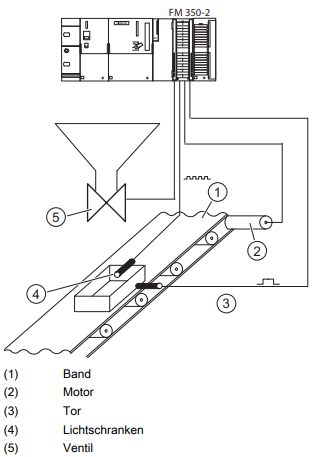
\includegraphics[width=0.8\textwidth]{Fotos/Beispiel_fm350-2.png}
    \caption{Beispiel für den Einsatz einer FM 350-2 in der S7-300 \cite{fm350_Handbuch}}
    \label{fig:fm350-2}
\end{figure}



%//////////////////////////////////////////////////////////////////////////////////////////////////////////////////////
%//////////////////////////////////////////////////////////////////////////////////////////////////////////////////////
\section{Vorteile und neue Möglichkeiten durch das TM FAST Modul} 

%//////////////////////////////////////////////////////////////////////////////////////////////////////////////////////
%//////////////////////////////////////////////////////////////////////////////////////////////////////////////////////
\section{Anforderungen an die Neuentwicklung} 


\begin{table}[h]
    \centering
    \renewcommand{\arraystretch}{1.3}
    \begin{tabularx}{\textwidth}{|X|X|X|}
        \hline
        \textbf{Kriterium} & \textbf{TM FAST} & \textbf{FM 350-2} \\
        \hline
        \multicolumn{3}{|c|}{\textbf{Unterschiede}} \\
        \hline
        Architektur & FPGA-basiert, flexible und programmierbare Hardwareplattform & Reines Zählermodul ohne FPGA-Technologie \\
        \hline
        Funktionalität & Kann komplexe Prozesssteuerungs- und Überwachungsaufgaben übernehmen & Spezialisiert auf Zählen, Frequenz- und Drehzahlmessung \\
        \hline
        Prozessintegration & Kann direkt in den Produktionsprozess eingreifen und Prozessalarme auslösen & Liefert Zähler- und Messwerte, die von der übergeordneten Steuerung weiterverarbeitet werden \\
        \hline
        Flexibilität & Hohe Flexibilität und Anpassungsfähigkeit durch FPGA-Architektur & Festgelegte Funktionalität, die nicht ohne Weiteres erweitert werden kann \\
        \hline
        \multicolumn{3}{|c|}{\textbf{Gemeinsamkeiten}} \\
        \hline
        Zählfunktionen & \multicolumn{2}{c|}{Beide Module bieten Zählfunktionen mit hoher Auflösung (z.B. 32-Bit Zähltiefe)} \\
        \hline
        Frequenz- und Drehzahlmessung & \multicolumn{2}{c|}{Beide Module unterstützen die Messung von Frequenzen und Drehzahlen} \\
        \hline
        Einbindung in Steuerungsarchitektur & \multicolumn{2}{c|}{Beide Module werden in die übergeordnete Steuerungsarchitektur integriert} \\
        \hline
        Industrielle Anwendungen & \multicolumn{2}{c|}{Beide Module finden Einsatz in ähnlichen Industriebereichen wie Verpackung, Sortierung, Dosierung etc.} \\
        \hline
    \end{tabularx}
    \caption{Vergleich zwischen TM FAST und FM 350-2}
    \label{tab:tm_fast_vs_fm350-2}
\end{table}

% \begin{table}[h]     funktioniert
%     \centering
%     \renewcommand{\arraystretch}{1.3} % Erhöht den Zeilenabstand leicht
%     \begin{tabularx}{\textwidth}{|X|X|X|}
%         \hline
%         \textbf{Kriterium} & \textbf{TM FAST} & \textbf{FM 350-2} \\\multicolumn{3}{|c|}{\textbf{Unterschiede}} \\
%         \hline
%         Architektur & FPGA-basiert, flexible und programmierbare Hardwareplattform & Reines Zählermodul ohne FPGA-Technologie \\
%         \hline
%         Funktionalität & Kann komplexe Prozesssteuerungs- und Überwachungsaufgaben übernehmen & Spezialisiert auf Zählen, Frequenz- und Drehzahlmessung \\
%         \hline
%         Prozessintegration & Kann direkt in den Produktionsprozess eingreifen und Prozessalarme auslösen & Liefert Zähler- und Messwerte, die von der übergeordneten Steuerung weiterverarbeitet werden \\
%         \hline
%         Flexibilität & Hohe Flexibilität und Anpassungsfähigkeit durch FPGA-Architektur & Festgelegte Funktionalität, die nicht ohne Weiteres erweitert werden kann \\
%         \hline
%     \end{tabularx}
%     \caption{Vergleich zwischen TM FAST und FM 350-2}
%     \label{tab:tm_fast_vs_fm350-2}
% \end{table}


